\section{System Model}
The software architecture follows the one proposed in "\textit{Guide for the Use
of Ada Ravenscar Profile in High Integrity Systems}"
\cite{burnsGuideUseAda2004}. It is comprised by one periodic producer task that
can activate two other sporadic tasks. Additionally, there is a sporadic event
server that manages the occurrence of external events. In the implemented
application events are generated by a periodic task that emulate user
interaction, for repeatability reasons. 

Table [\ref{tab:tasks-list}] contains the list of tasks constituting the
application, together with their typology, deadline, period (if applicable) and
priority. Priorities have been assigned using the \textit{Deadline Monotonic}
algorithm, which assigns priorities in decreasing order, starting with jobs of
smaller relative deadline. It is an optimal algorithm for constrained deadlines
and fixed-priority scheduling \cite[p.~119]{liuRealTimeSystems2000}. \\ 
The deadline watchdogs have been given the highest priority in order to detect
overrun without interference from other tasks (see section
\ref{sec:DeadlineMissDetection} for furhter details).

The tasks in the system share various resources. Access is regulated by variants
of the \textit{Priority Ceiling Protocol}
\cite{shaPriorityInheritanceProtocols1990} depending on the implementation: the
Ada system implements the \textit{Immediate Priority Ceiling Protocol}
\cite{chengImplementationPriorityCeiling2007}, while the Rust system uses
\textit{Stack Resource Policy} \cite{bakerStackbasedSchedulingRealtime1991}.\\ 
While the implementation is slightly different, both protocols show the same
properties and response-time behavior. They require to specify the ceiling value
for each shared resource, which is obtained by picking the maximum priority
value among all the task using the given resource. 

Table [\ref{tab:res-list}] contains the list of all the shared resources in the
system, together with their users (tasks) and their priority ceiling. 

\begin{table*}[!t]
  \centering
    \begin{tabular}{p{0.2\linewidth} p{0.2\linewidth} p{0.1\linewidth}
    p{0.2\linewidth} p{0.1\linewidth}}
      \hline
        \textbf{Task} & \textbf{Task Type} & \textbf{Period (ms)} & 
        \textbf{Deadline (ms)} & \textbf{Priority} \\
      \hline
        Activation Log Reader & Sporadic & 3000 & 1000 & 3\\
        On Call Producer & Sporadic & 5000 & 800 & 5 \\
        Regular Producer & Periodic & 1000 & 500 & 7 \\
        External Event Server & Sporadic (interrupt) & 5000 & 100 & 11 \\
        Interrupt Generator & Periodic & 5000 & 50 & 13 \\
        ALR Deadline Watchdog & Sporadic & 3000 & 1000 & 15 \\
        OCP Deadline Watchdog  & Sporadic & 5000 & 800 & 15 \\
        RP Deadline Watchdog & Periodic & 1000 & 500 & 15 \\
        EES Deadline Watchdog & Sporadic (interrupt) & 5000 & 100 & 15 \\
      \hline
    \end{tabular}
  \caption[Task Table]{List of tasks in the system, with their parameters}
  \label{tab:tasks-list}
\end{table*}

\begin{table*}[!t]
  \centering
  \begin{tabular}{ p{0.2\linewidth} p{0.5\linewidth} p{0.1\linewidth}}
    \hline
    \textbf{Resource} & \textbf{Users} & \textbf{Ceiling}\boldmath{$\pi_R$} \\
    \hline
    Activation Log & Activation Log Reader, External Event Server & 11 \\
    Event Queue & External Event Server, External Event ISR & 11 \\
    Request Buffer & Regular Producer, On-Call Producer & 7 \\
    ALR Deadline Object & Activation Log Reader, ALR Deadline Watchdog & 15 \\
    OCP Deadline Object & On-Call Producer, OCP Deadline Watchdog & 15 \\
    RP Deadline Object & Regular Producer, RP Deadline Watchdog & 15 \\
    EES Deadline Object & External Event Server, EES Deadline Watchdog & 15 \\
    \hline  
  \end{tabular}
  \caption[Resource table]{List of shared resources in the system, with their 
  users and priority ceilings} 
  \label{tab:res-list}
\end{table*}

In order to emulate a realistic workload for task requiring some kind of
computation, the small variant of the Whetstone benchmark
\cite{curnowSyntheticBenchmark1976} is used. It includes different kind of
computations: integer, floating-point, trigonometry, branches and function
calls, with the aim of testing the system under a wide range of loads. \\ 
This workload is a parameter that we used in the analysis section to create
different workload levels and observe the resulting behavior of the system,
first by simulating it using the MAST tool \cite{MASTComprehensiveTool}, then by
running the application in a real setting.

To this end, we have used the \textit{Olimex STM32\-H405} \cite{olimexSTM32H405}
development board, together with a \textit{STLink\-v2} \cite{STLINKV2Tool}
debugging probe. 

\subsection{Tasks Description}

\subsubsection{Activation Log Reader}

The \textit{Activation Log Reader} is a sporadic task which awaits on a signal
received from the \textit{Regular Producer}, and then performs its internal
operation which consists of an artificial Whetstone workload, followed by a
reading of the status of the \textit{Activation Log} and a print that notifies
the end of its sporadic activation.

\subsubsection{On-Call Producer}

The \textit{On-Call Producer} is a sporadic task that waits for a request
deposit into the \textit{Request Buffer}, then reads it and runs a Whetstone
workload with load equal to the extracted value. The requests are sent by the
\textit{Regular Producer}, and they are meant to represent a scenario in which a
main task delegates some work to a helper task in the event of an overload. 

\subsubsection{Regular Producer}

The \textit{Regular Producer} is a periodic task that runs a Whetstone workload
with a predefined load value, then, based on a predetermined criterion, can
release the \textit{Activation Log Reader} and send a work request to the
\textit{On-Call Producer}. 

\subsubsection{External Event Server}

The \textit{External Event Server} is a sporadic task that waits for events put
onto the \textit{Event Queue} by the interrupt handler bound to the simulated
external event. It updates the \textit{Activation Log} counter on each
activation. 

\subsubsection{Deadline Watchdogs}

For every task in the system there is a watchdog monitor task that checks for
deadline overruns. It has the maximum priority to prevent interference. It
maintains the number of deadline misses and whenever it detects one 
it prints a warning message (see section \ref{sec:DeadlineMissDetection} for
further details). \\

\noindent Figure [\ref{fig:system-architecture}] shows a high-level view of the system
architecture 

\begin{figure}[t]
  \centering
  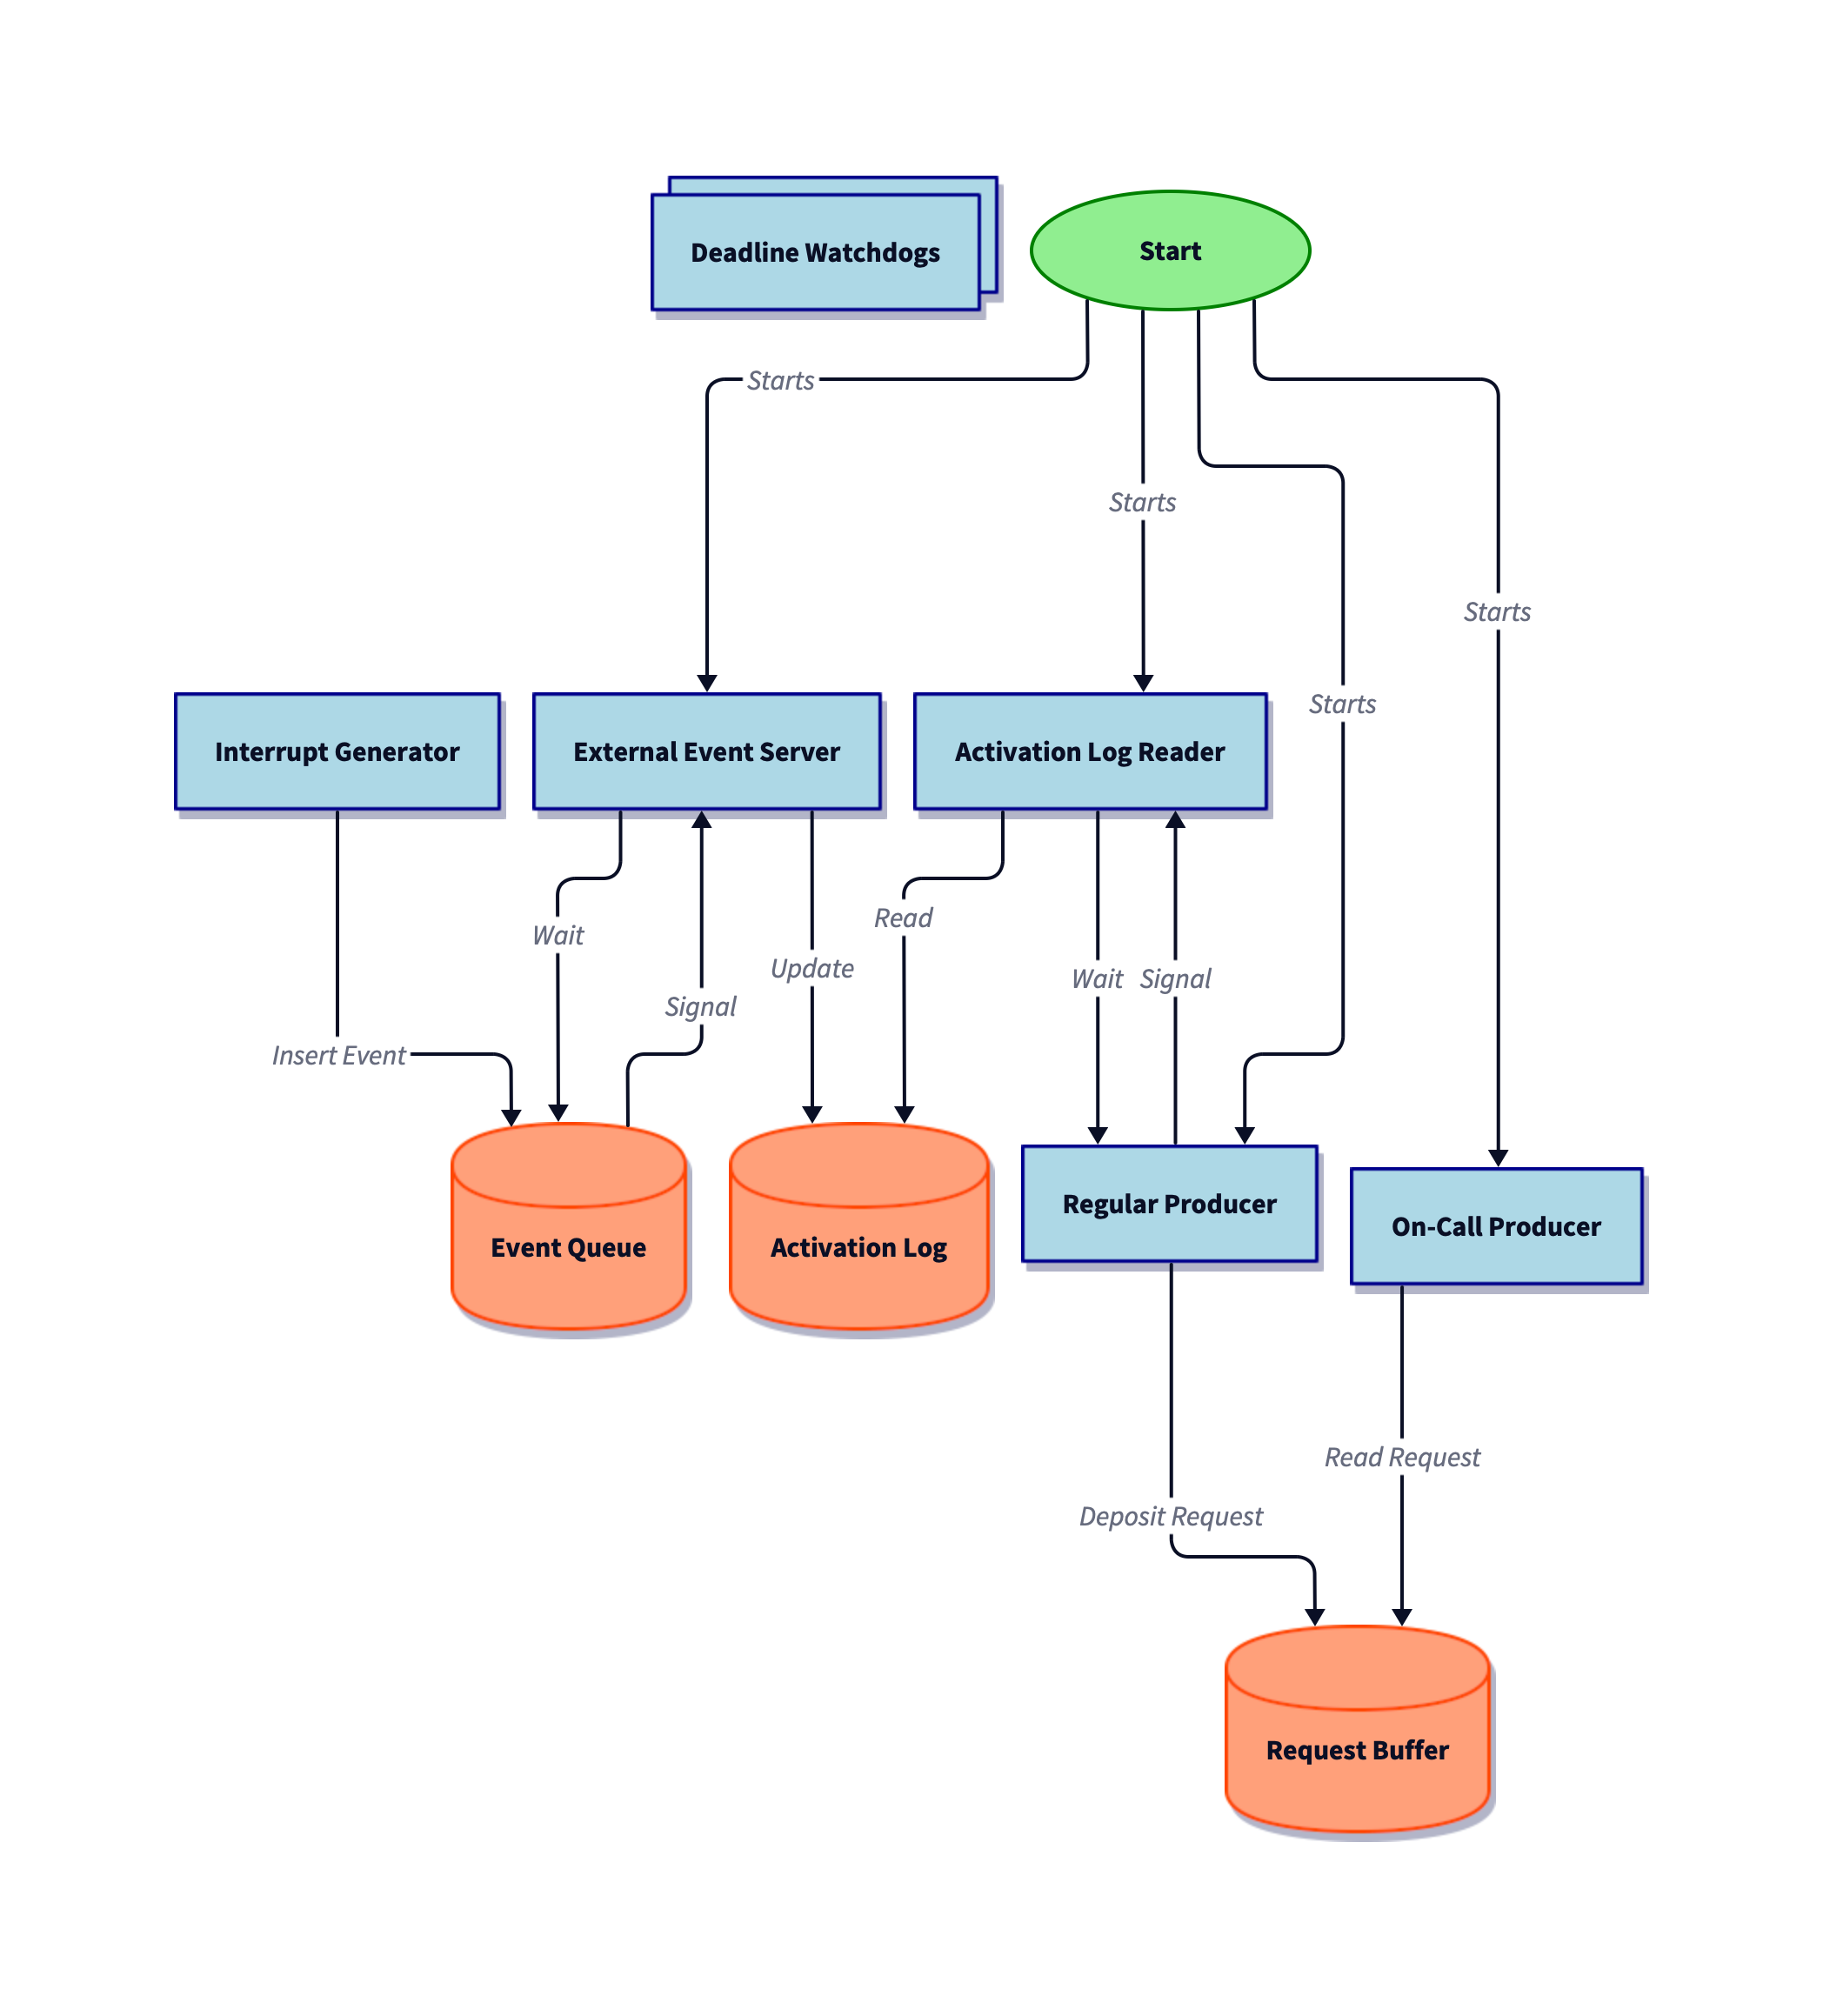
\includegraphics[width=0.45\textwidth]{images/system-diagram.png}
  \caption[System architecture]{System architecture diagram}
  \label{fig:system-architecture}
\end{figure}